% !TeX Options = -shell-escape
\documentclass{panicsoftware-presentation}

\usepackage{tikz}
\usetikzlibrary{decorations.pathreplacing}

\title{Lifetime of the C++ object?}
\author{Dawid Pilarski}
\date{}

\institute{dawid.pilarski@tomtom.com \\ dawid.pilarski@panicsoftware.com \\ \href{http://blog.panicsoftware.com}{blog.panicsoftware.com} }

\newenvironment{itemizeSeq}{\begin{itemize}[<+-|alert@+>]}{\end{itemize}}
\newenvironment{itemizeNColorSeq}{\begin{itemize}[<+->]}{\end{itemize}}

\begin{document}

\begin{frame}
	\maketitle
\end{frame}

\begin{frame}{Agenda}
	\tableofcontents
\end{frame}

\begin{frame}{Who am I?}
			\centering \alert{Dawid Pilarski}
			\vskip 1em
	\begin{columns}[onlytextwidth]
		\begin{column}{0.7\textwidth}
			\begin{itemize}
				\item Senior Software Developer in TomTom
				\item Member of the ISO/JTC1/SC22/WG21
				\item Member of the PKN KT {\tiny(programming languages)}
				\item C++ blog writer
			\end{itemize}
		\end{column}
		\begin{column}{0.29\textwidth}
				
\includegraphics[width=\linewidth]{Dawid_Pilarski.jpg}				
		\end{column}	
	\end{columns}
\end{frame}

\begin{frame}{Questions.}
	
	\vfill
	\centerline{Questions...}
	\vfill

\end{frame}

\begin{frame}{Question...}

\centerline{Do you think we are going to talk about \alert{basics}?}

\end{frame}

\begin{frame}{What we talk about are basics.}

	\centering
	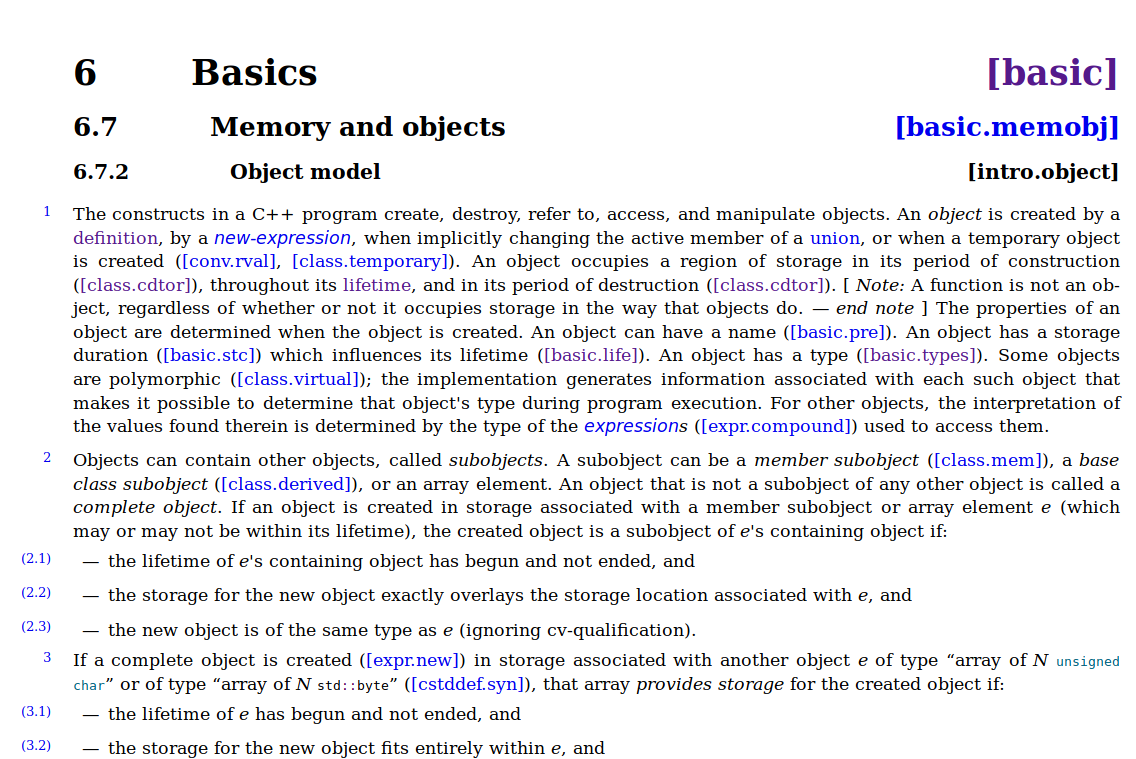
\includegraphics[width=1.0\linewidth]{graphics/objects_basics.png}

\end{frame}


\section{Theory}

\begin{frame}{Title decomposition}

\centerline{What's the \only{lifetime}<1>\only{\alert{lifetime}}<2-> of your \only{object}<1-2>\only{\alert{object}}<3>?}
\pause
\begin{itemizeSeq}
	\item What is a lifetime?
	\item What is an object?
\end{itemizeSeq}

\end{frame}

\section*{Objects}

\begin{frame}{The object}

Objects are:
\begin{itemize}
	\item created
	\item destroyed
	\item refered to
	\item accessed
	\item manipulated
\end{itemize}

\end{frame}

\begin{frame}{The Object}

\begin{columns}[T]
	\begin{column}{0.58\linewidth}
	
	Is created:
	\begin{itemizeSeq}
		\item by the definition
		\item by the new expression
		\item when changing active\\ member of a union
		\item by creation of the temporary
	\end{itemizeSeq}
	\end{column}

	\begin{column}{0.48\linewidth}
	
	\only{\centering\inputminted{\myCpp}{examples/object-definition.cpp}}<1>
	\only{\centering\inputminted{\myCpp}{examples/new-expression.cpp}}<2>
	\only{\centering\inputminted{\myCpp}{examples/union-active-member-change.cpp}}<3>
	\only{\centering\inputminted{\myCpp}{examples/temporary-creation.cpp}}<4>
	\end{column}

\end{columns}

\end{frame}


\newcounter{tmpCounter}
\begin{frame}{The object}

\begin{columns}
\begin{column}{0.3\linewidth}

Has:
\begin{itemizeSeq}
	\item optional name
	\item storage and it's duration
	\begin{itemizeSeq}
		\item static
		\item thread
		\item automatic
		\item dynamic
	\end{itemizeSeq}
	\item lifetime
	\item type
\end{itemizeSeq}

\end{column}

\begin{column}{0.5\linewidth}
\only{\alert{program duration}}<3>
\only{\alert{thread duration}}<4>
\only{\alert{enclosing scope duration}}<5>
\only{\alert{controlled by user}}<6>
\end{column}

\end{columns}
\end{frame}

\begin{frame}{The object}

\centerline{Is not a reference {\scriptsize(although reference has lifetime)}}

\end{frame}

\begin{frame}[fragile]{The variable}

\centerline{Is created by a \alert{declaration} of an \alert{object} or the \alert{reference}.}
\pause
\vfill

\begin{columns}[t]

\begin{column}{0.3\linewidth}
\begin{minted}{\myCpp}
int x;
\end{minted}
\vskip 1cm
Is a variable.

\end{column}
\pause

\begin{column}{0.3\linewidth}
\begin{minted}{\myCpp}
int& x = ...
\end{minted}
\vskip 1cm
Is variable.

\end{column}
\pause

\begin{column}{0.3\linewidth}
\begin{minted}{\myCpp}
struct X{int z;}x;
\end{minted}
\vskip 1cm
Neither \texttt{X} nor \texttt{z} are variables.\\
\texttt{x} is a variable.
\end{column}

\end{columns}

\end{frame}

\begin{frame}{Summary: variable, reference, object}
\centering
\begin{figure}
\resizebox{0.9\linewidth}{!}{
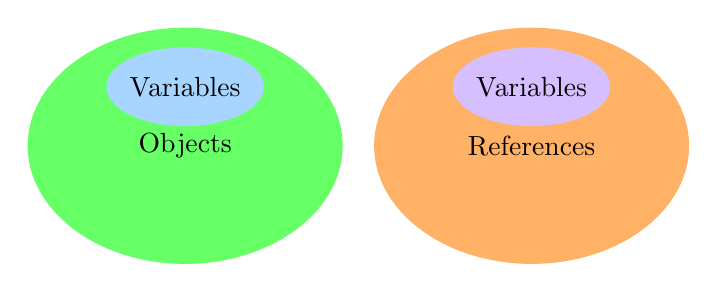
\begin{tikzpicture}
\begin{scope}[blend group=soft light]

\fill[blue!30!white] (-2.2,-0.25) circle[x radius=1cm, y radius=0.5cm];
\fill[blue!30!white] (2.2,-0.25) circle[x radius=1cm, y radius=0.5cm];
\fill[green!60!white] (-2.2,-1) circle[x radius=2cm, y radius=1.5cm];
\fill[orange!60!white] (2.2,-1) circle[x radius=2cm, y radius=1.5cm];

\end{scope}

\node at(-2.2,-0.25){Variables};
\node at(2.2,-0.25){Variables};
\node at(2.2,-1){References};
\node at(-2.2,-1){Objects};

\end{tikzpicture}}

\end{figure}

\end{frame}


\begin{frame}{Summary: variable, reference, object}
	Just in case you want to check validity with the \href{http://cppreference.com}{\alert{cppreference}}:

	\begin{itemizeSeq}
		\item The object has been recently updated.
		\item The variable definition is unmaintained and unsupported.
		\item Same about references...
	\end{itemizeSeq}
\end{frame}

\section*{Lifetime}

\begin{frame}{What is a lifetime?}

\centerline{Lifetime is a \alert{runtime} property of an object.}

\vfill
\centering

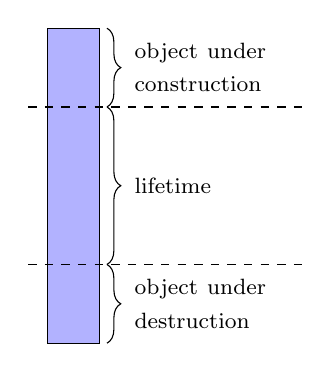
\begin{tikzpicture}

\draw[fill=blue!30!white] (-.75, -2) rectangle (-0.1, 2);

\draw[dashed] (-1, 1) -- (2.5, 1);
\draw[dashed] (-1, -1) -- (2.5, -1);

\draw [decorate, decoration={brace, amplitude=5pt}] (0, 2) -- (0, 1) node[xshift=1.35cm ,midway, text width=2cm]{\footnotesize object under construction};
\draw [decorate, decoration={brace, amplitude=5pt}] (0, 1) -- (0,-1) node[xshift=1.35cm ,midway, text width=2cm]{\footnotesize lifetime};
\draw [decorate, decoration={brace, amplitude=5pt}] (0, -1) -- (0, -2) node[xshift=1.35cm ,midway, text width=2cm]{\footnotesize object under destruction};;

\end{tikzpicture}
\vfill
\centerline{During the lifetime of an object you can use it without additional restrictions.}

\end{frame}

\begin{frame}{When does the lifetime start?}

\centerline{The lifetime of an object \alert{starts}, when:}

\begin{itemizeSeq}

\item storage with the proper alignment and size for type T is obtained
\item its initialization \alert{(if any)} is complete
\item if the object is a union member or subobject thereof, its lifetime only begins if that union member is the initialized member

\end{itemizeSeq}
\end{frame}

\begin{frame}{When does the lifetime end?}

\centerline{The lifetime of an object \alert{ends}, when:}

\begin{itemizeSeq}

\item object is destroyed (for non class types),
\item destructor is called (for the class types), or
\item storage occupied by an object is reused or released.

\end{itemizeSeq}
\end{frame}

\section{Object model intuition}

\begin{frame}{The usual mindset towards object}

\begin{itemizeSeq}
\item We have got a memory
\item Objects are the way to represent value in that memory
\end{itemizeSeq}


TODO: Examples/illustrations

\end{frame}

\begin{frame}{Examples of invalid C++}

TODO: example with reinterpret\_casting piece of memory to the object

TODO: example with type punning on unions

\end{frame}

\begin{frame}{Special case, when it's correct}

TODO example with 2 standard layout structs

\end{frame}

\begin{frame}{Compiler thinks in terms of objects and types}

Why above is wrong?
because the title

\end{frame}

\begin{frame}{Assumptions, that compiler does}

examples with assembly why this assumption is important

\end{frame}

\begin{frame}{More examples with wrong usages}

\end{frame}

\begin{frame}{std::launder}

\end{frame}

\begin{frame}{Evolution of the rules}

pre C++11 (make sure it's correct).

Cannot create object in the same type in the same place as previous object

\end{frame}

\begin{frame}{Evolution of the rules}
After C++ 11 (check)

You can create an object of the same type as long as there are no references and const objects

\end{frame}

\begin{frame}{Evolution of the rules}

Since C++20

You can create object of the same type.

\end{frame}

\begin{frame}{Implicit object creation in C++20}

\end{frame}

\section{Beyond the object lifetime.}

\begin{frame}{Before birth}

\end{frame}

\begin{frame}{Delayed members initialization}

\end{frame}

\begin{frame}{Concurrent access and vptr}

\end{frame}

\begin{frame}{dynamic\_cast and type\_id}

\end{frame}

\begin{frame}{Afterlife}

\end{frame}

\begin{frame}{vptr and synchronization in the destructor}

\end{frame}

\begin{frame}{Immortality}

\end{frame}


\end{document}